\documentclass[11pt,]{article}
\usepackage[left=1in,top=1in,right=1in,bottom=1in]{geometry}
\newcommand*{\authorfont}{\fontfamily{phv}\selectfont}
  \usepackage[]{mathpazo}
  
  
  \usepackage[T1]{fontenc}
\usepackage[utf8]{inputenc}



\usepackage{abstract}
\renewcommand{\abstractname}{}    % clear the title
\renewcommand{\absnamepos}{empty} % originally center

\renewenvironment{abstract}
{{%
  \setlength{\leftmargin}{0mm}
  \setlength{\rightmargin}{\leftmargin}%
}%
  \relax}
{\endlist}

\makeatletter
\def\@maketitle{%
  \newpage
  %  \null
  %  \vskip 2em%
    %  \begin{center}%
    \let \footnote \thanks
  {\fontsize{18}{20}\selectfont\raggedright  \setlength{\parindent}{0pt} \@title \par}%
}
%\fi
\makeatother


  
  
  \setcounter{secnumdepth}{0}

      \usepackage{color}
  \usepackage{fancyvrb}
  \newcommand{\VerbBar}{|}
  \newcommand{\VERB}{\Verb[commandchars=\\\{\}]}
  \DefineVerbatimEnvironment{Highlighting}{Verbatim}{commandchars=\\\{\}}
  % Add ',fontsize=\small' for more characters per line
  \usepackage{framed}
  \definecolor{shadecolor}{RGB}{248,248,248}
  \newenvironment{Shaded}{\begin{snugshade}}{\end{snugshade}}
  \newcommand{\AlertTok}[1]{\textcolor[rgb]{0.94,0.16,0.16}{#1}}
  \newcommand{\AnnotationTok}[1]{\textcolor[rgb]{0.56,0.35,0.01}{\textbf{\textit{#1}}}}
  \newcommand{\AttributeTok}[1]{\textcolor[rgb]{0.77,0.63,0.00}{#1}}
  \newcommand{\BaseNTok}[1]{\textcolor[rgb]{0.00,0.00,0.81}{#1}}
  \newcommand{\BuiltInTok}[1]{#1}
  \newcommand{\CharTok}[1]{\textcolor[rgb]{0.31,0.60,0.02}{#1}}
  \newcommand{\CommentTok}[1]{\textcolor[rgb]{0.56,0.35,0.01}{\textit{#1}}}
  \newcommand{\CommentVarTok}[1]{\textcolor[rgb]{0.56,0.35,0.01}{\textbf{\textit{#1}}}}
  \newcommand{\ConstantTok}[1]{\textcolor[rgb]{0.00,0.00,0.00}{#1}}
  \newcommand{\ControlFlowTok}[1]{\textcolor[rgb]{0.13,0.29,0.53}{\textbf{#1}}}
  \newcommand{\DataTypeTok}[1]{\textcolor[rgb]{0.13,0.29,0.53}{#1}}
  \newcommand{\DecValTok}[1]{\textcolor[rgb]{0.00,0.00,0.81}{#1}}
  \newcommand{\DocumentationTok}[1]{\textcolor[rgb]{0.56,0.35,0.01}{\textbf{\textit{#1}}}}
  \newcommand{\ErrorTok}[1]{\textcolor[rgb]{0.64,0.00,0.00}{\textbf{#1}}}
  \newcommand{\ExtensionTok}[1]{#1}
  \newcommand{\FloatTok}[1]{\textcolor[rgb]{0.00,0.00,0.81}{#1}}
  \newcommand{\FunctionTok}[1]{\textcolor[rgb]{0.00,0.00,0.00}{#1}}
  \newcommand{\ImportTok}[1]{#1}
  \newcommand{\InformationTok}[1]{\textcolor[rgb]{0.56,0.35,0.01}{\textbf{\textit{#1}}}}
  \newcommand{\KeywordTok}[1]{\textcolor[rgb]{0.13,0.29,0.53}{\textbf{#1}}}
  \newcommand{\NormalTok}[1]{#1}
  \newcommand{\OperatorTok}[1]{\textcolor[rgb]{0.81,0.36,0.00}{\textbf{#1}}}
  \newcommand{\OtherTok}[1]{\textcolor[rgb]{0.56,0.35,0.01}{#1}}
  \newcommand{\PreprocessorTok}[1]{\textcolor[rgb]{0.56,0.35,0.01}{\textit{#1}}}
  \newcommand{\RegionMarkerTok}[1]{#1}
  \newcommand{\SpecialCharTok}[1]{\textcolor[rgb]{0.00,0.00,0.00}{#1}}
  \newcommand{\SpecialStringTok}[1]{\textcolor[rgb]{0.31,0.60,0.02}{#1}}
  \newcommand{\StringTok}[1]{\textcolor[rgb]{0.31,0.60,0.02}{#1}}
  \newcommand{\VariableTok}[1]{\textcolor[rgb]{0.00,0.00,0.00}{#1}}
  \newcommand{\VerbatimStringTok}[1]{\textcolor[rgb]{0.31,0.60,0.02}{#1}}
  \newcommand{\WarningTok}[1]{\textcolor[rgb]{0.56,0.35,0.01}{\textbf{\textit{#1}}}}
        
    \usepackage{graphicx,grffile}
\makeatletter
\def\maxwidth{\ifdim\Gin@nat@width>\linewidth\linewidth\else\Gin@nat@width\fi}
\def\maxheight{\ifdim\Gin@nat@height>\textheight\textheight\else\Gin@nat@height\fi}
\makeatother
% Scale images if necessary, so that they will not overflow the page
% margins by default, and it is still possible to overwrite the defaults
% using explicit options in \includegraphics[width, height, ...]{}
\setkeys{Gin}{width=\maxwidth,height=\maxheight,keepaspectratio}
  
    \title{Homework 3  }
  
  
  
  \author{\Large Joyce Yu Cahoon\vspace{0.05in} \newline\normalsize\emph{}  }
  
  
  \date{}

\usepackage{titlesec}

\titleformat*{\section}{\normalsize\bfseries}
\titleformat*{\subsection}{\normalsize\itshape}
\titleformat*{\subsubsection}{\normalsize\itshape}
\titleformat*{\paragraph}{\normalsize\itshape}
\titleformat*{\subparagraph}{\normalsize\itshape}


  
      
  
  \newtheorem{hypothesis}{Hypothesis}
\usepackage{setspace}

\makeatletter
\@ifpackageloaded{hyperref}{}{%
  \ifxetex
  \PassOptionsToPackage{hyphens}{url}\usepackage[setpagesize=false, % page size defined by xetex
                                                 unicode=false, % unicode breaks when used with xetex
                                                 xetex]{hyperref}
  \else
    \PassOptionsToPackage{hyphens}{url}\usepackage[unicode=true]{hyperref}
  \fi
}

\@ifpackageloaded{color}{
  \PassOptionsToPackage{usenames,dvipsnames}{color}
}{%
  \usepackage[usenames,dvipsnames]{color}
}
\makeatother
\hypersetup{breaklinks=true,
bookmarks=true,
pdfauthor={Joyce Yu Cahoon ()},
pdfkeywords = {},  
pdftitle={Homework 3},
colorlinks=true,
citecolor=blue,
urlcolor=blue,
linkcolor=magenta,
pdfborder={0 0 0}}
\urlstyle{same}  % don't use monospace font for urls

% set default figure placement to htbp
\makeatletter
\def\fps@figure{htbp}
\makeatother

\setlength{\abovedisplayskip}{.2pt}
\setlength{\belowdisplayskip}{.2pt}
\usepackage{placeins}
\usepackage{setspace}
\usepackage{chngcntr}
\usepackage{multicol}
\usepackage{lscape}
\counterwithin{figure}{section}
\counterwithin{table}{section}
\usepackage{mathrsfs}
\usepackage{mathtools}
\usepackage{multirow}
\newtheorem{theorem}{Theorem}
\usepackage[linesnumbered,algoruled,boxed,lined,commentsnumbered]{algorithm2e}
\usepackage{bm}
\usepackage{framed}
\usepackage{xcolor}
\let\oldquote=\quote
\let\endoldquote=\endquote
\colorlet{shadecolor}{orange!15}
\renewenvironment{quote}{\begin{shaded*}}{\end{shaded*}}
\newcommand{\minus}{\scalebox{0.75}[1.0]{$-$}}
\newcommand{\V}[1]{{\bm{{#1}}}}


% add tightlist ----------
\providecommand{\tightlist}{%
\setlength{\itemsep}{0pt}\setlength{\parskip}{0pt}}

\begin{document}

% \pagenumbering{arabic}% resets `page` counter to 1 
%
% \maketitle

{% \usefont{T1}{pnc}{m}{n}
\setlength{\parindent}{0pt}
\thispagestyle{plain}
{\fontsize{18}{20}\selectfont\raggedright 
\maketitle  % title \par  

}

{
  \vskip 13.5pt\relax \normalsize\fontsize{11}{12} 
  \textbf{\authorfont Joyce Yu Cahoon} \hskip 15pt \emph{\small }   
  
}

}






\vskip 6.5pt


\noindent  \hypertarget{section}{%
\section{7.1}\label{section}}

What is the gross exposure of the portfolio with weights: \[
{\bm{{w}}} = (-0.2, 0.3, 0.4, -0.2, 0.1, 0.2, 0, 0.4)
\] What is the risk of this portfolio invested on ``Dell'', ``Ford'',
``GE'', ``IBM'', ``J\&J'', ``Merck'', ``3 mo Treasury'', ``S\&P500'' in
past ten years (January 1, 2005 to January 1, 2015 using daily data).
Compare it with the portfolio with equal weight.

\begin{quote}
The gross exposure can be calculated simply as:
\end{quote}

\begin{Shaded}
\begin{Highlighting}[]
\NormalTok{w <-}\StringTok{ }\KeywordTok{c}\NormalTok{(}\OperatorTok{-}\FloatTok{0.2}\NormalTok{, }\FloatTok{0.3}\NormalTok{, }\FloatTok{0.4}\NormalTok{, }\FloatTok{-0.2}\NormalTok{, }\FloatTok{0.1}\NormalTok{, }\FloatTok{0.2}\NormalTok{, }\DecValTok{0}\NormalTok{, }\FloatTok{0.4}\NormalTok{)}
\KeywordTok{sum}\NormalTok{(}\KeywordTok{abs}\NormalTok{(w))}
\end{Highlighting}
\end{Shaded}

\begin{verbatim}
## [1] 1.8
\end{verbatim}

\begin{quote}
The gross exposure with equal weights is:
\end{quote}

\begin{Shaded}
\begin{Highlighting}[]
\NormalTok{w <-}\StringTok{ }\KeywordTok{rep}\NormalTok{(}\DecValTok{1}\NormalTok{, }\KeywordTok{length}\NormalTok{(w))}\OperatorTok{/}\KeywordTok{length}\NormalTok{(w)}
\KeywordTok{sum}\NormalTok{(}\KeywordTok{abs}\NormalTok{(w))}
\end{Highlighting}
\end{Shaded}

\begin{verbatim}
## [1] 1
\end{verbatim}

\begin{quote}
To calculate the risk of the original portfolio. First, we obtain the
data we need. Note that we remove ``DELL'' as that is not provided from
Yahoo!Finance:
\end{quote}

\begin{Shaded}
\begin{Highlighting}[]
\CommentTok{# load the necessary financial data from quantmod }
\KeywordTok{library}\NormalTok{(quantmod)}
\NormalTok{start <-}\StringTok{ }\KeywordTok{as.Date}\NormalTok{(}\StringTok{"2005-01-01"}\NormalTok{)}
\NormalTok{end <-}\StringTok{ }\KeywordTok{as.Date}\NormalTok{(}\StringTok{"2015-01-01"}\NormalTok{)}
\NormalTok{assets <-}\StringTok{ }\KeywordTok{c}\NormalTok{(}\CommentTok{# "DVMT" # DELL is DROPPED since not provided by Quantmod}
  \StringTok{"F"}\NormalTok{, }
  \StringTok{"GE"}\NormalTok{, }
  \StringTok{"IBM"}\NormalTok{, }
  \StringTok{"JNJ"}\NormalTok{,}
  \StringTok{"MRK"}\NormalTok{,}
  \StringTok{"SPY"}\NormalTok{)}
\KeywordTok{getSymbols}\NormalTok{(assets, }\DataTypeTok{from =}\NormalTok{ start, }\DataTypeTok{to =}\NormalTok{ end) }
\CommentTok{# get the 3 mo tresury data }
\KeywordTok{getSymbols}\NormalTok{(}\StringTok{"DGS3MO"}\NormalTok{, }\DataTypeTok{src =} \StringTok{"FRED"}\NormalTok{)}
\CommentTok{# merge into one df }
\NormalTok{closing.prices <-}\StringTok{ }\KeywordTok{merge.xts}\NormalTok{(DGS3MO, }
\NormalTok{                            F[, }\DecValTok{4}\NormalTok{], }
\NormalTok{                            GE[, }\DecValTok{4}\NormalTok{],}
\NormalTok{                            IBM[, }\DecValTok{4}\NormalTok{], }
\NormalTok{                            JNJ[, }\DecValTok{4}\NormalTok{], }
\NormalTok{                            MRK[, }\DecValTok{4}\NormalTok{], }
\NormalTok{                            SPY[, }\DecValTok{4}\NormalTok{])}
\CommentTok{# save as RDS }
\KeywordTok{saveRDS}\NormalTok{(closing.prices, }\StringTok{"~/workspace/st790-financial-stats/hw4/closing.rds"}\NormalTok{)}
\end{Highlighting}
\end{Shaded}

\begin{quote}
With the daily log returns, we can then find:
\end{quote}

\begin{Shaded}
\begin{Highlighting}[]
\NormalTok{dat <-}\StringTok{ }\KeywordTok{readRDS}\NormalTok{(}\StringTok{"~/workspace/st790-financial-stats/hw4/closing.rds"}\NormalTok{)}
\CommentTok{# filter out the information for the timeframe of interest }
\NormalTok{data <-}\StringTok{ }\NormalTok{dat[}\StringTok{"2005-01-01/2015-01-01"}\NormalTok{]}
\NormalTok{data <-}\StringTok{ }\KeywordTok{na.omit}\NormalTok{(data)}
\CommentTok{# get daily log returns }
\NormalTok{by_day <-}\StringTok{ }\KeywordTok{data.frame}\NormalTok{() }
\ControlFlowTok{for}\NormalTok{(i }\ControlFlowTok{in} \DecValTok{1}\OperatorTok{:}\KeywordTok{ncol}\NormalTok{(data))\{}
\NormalTok{  temp <-}\StringTok{ }\NormalTok{data[, i]}
\NormalTok{  daily <-}\StringTok{ }\KeywordTok{log}\NormalTok{(}\KeywordTok{dailyReturn}\NormalTok{(temp)}\OperatorTok{+}\DecValTok{1}\NormalTok{)}
\NormalTok{  by_day <-}\StringTok{ }\KeywordTok{cbind}\NormalTok{(by_day, daily)}
  \KeywordTok{colnames}\NormalTok{(by_day)[i] <-}\StringTok{ }\KeywordTok{strsplit}\NormalTok{(}\KeywordTok{names}\NormalTok{(temp), }\StringTok{"[.]"}\NormalTok{)[[}\DecValTok{1}\NormalTok{]][}\DecValTok{1}\NormalTok{]}
\NormalTok{\}}
\CommentTok{# get the excess return }
\NormalTok{excess_return <-}\StringTok{ }\KeywordTok{data.frame}\NormalTok{()}
\ControlFlowTok{for}\NormalTok{(j }\ControlFlowTok{in} \DecValTok{2}\OperatorTok{:}\KeywordTok{ncol}\NormalTok{(by_day))\{}
\NormalTok{  temp <-}\StringTok{ }\NormalTok{by_day[, j] }\OperatorTok{-}\StringTok{ }\NormalTok{by_day[, }\DecValTok{1}\NormalTok{]}
\NormalTok{  excess_return <-}\StringTok{ }\KeywordTok{cbind}\NormalTok{(excess_return, temp)}
  \KeywordTok{colnames}\NormalTok{(excess_return)[j}\DecValTok{-1}\NormalTok{] <-}\StringTok{ }\KeywordTok{names}\NormalTok{(temp)}
\NormalTok{\}}
\CommentTok{# get the covariance matrix }
\NormalTok{r <-}\StringTok{ }\KeywordTok{cbind}\NormalTok{(by_day[,}\DecValTok{1}\NormalTok{], excess_return)}
\NormalTok{r[}\KeywordTok{is.infinite}\NormalTok{(r)] <-}\StringTok{ }\OtherTok{NA}
\NormalTok{r <-}\StringTok{ }\KeywordTok{na.omit}\NormalTok{(r)}
\NormalTok{Sigma <-}\StringTok{ }\KeywordTok{cov}\NormalTok{(r)}
\CommentTok{# weight vector given }
\NormalTok{w <-}\StringTok{ }\KeywordTok{c}\NormalTok{( }\FloatTok{0.3}\NormalTok{, }\FloatTok{0.4}\NormalTok{, }\FloatTok{-0.2}\NormalTok{, }\FloatTok{0.1}\NormalTok{, }\FloatTok{0.2}\NormalTok{, }\DecValTok{0}\NormalTok{, }\FloatTok{0.4}\NormalTok{)}
\NormalTok{w <-}\StringTok{ }\NormalTok{w}\OperatorTok{/}\KeywordTok{sum}\NormalTok{(w) }\CommentTok{# need to normalize since we removed DELL }
\CommentTok{# risk of portfolio }
\NormalTok{risk <-}\StringTok{ }\KeywordTok{sqrt}\NormalTok{(w }\OperatorTok\StringTok{ }\NormalTok{Sigma }\OperatorTok\StringTok{ }\NormalTok{w)}
\CommentTok{# print }
\KeywordTok{cat}\NormalTok{(}\StringTok{"The risk is: "}\NormalTok{, risk, }\StringTok{"}\CharTok{\textbackslash{}n}\StringTok{"}\NormalTok{)}
\end{Highlighting}
\end{Shaded}

\begin{verbatim}
## The risk is:  0.1148775
\end{verbatim}

\begin{Shaded}
\begin{Highlighting}[]
\CommentTok{# equal weight }
\NormalTok{w2 <-}\StringTok{ }\KeywordTok{rep}\NormalTok{(}\DecValTok{1}\NormalTok{, }\KeywordTok{length}\NormalTok{(w))}\OperatorTok{/}\KeywordTok{length}\NormalTok{(w)}
\CommentTok{# new risk }
\NormalTok{risk2 <-}\StringTok{ }\KeywordTok{sqrt}\NormalTok{(w2 }\OperatorTok\StringTok{ }\NormalTok{Sigma }\OperatorTok\StringTok{ }\NormalTok{w2)}
\CommentTok{# print }
\KeywordTok{cat}\NormalTok{(}\StringTok{"The new risk is: "}\NormalTok{, risk2, }\StringTok{"}\CharTok{\textbackslash{}n}\StringTok{"}\NormalTok{)}
\end{Highlighting}
\end{Shaded}

\begin{verbatim}
## The new risk is:  0.1633469
\end{verbatim}

\hypertarget{section-1}{%
\section{7.2}\label{section-1}}

Let \(X_1, \ldots, X_T\) be a sequence of stationary time series with
the autocovariance function \(\gamma(h) = cov(X_t, X_{t+h})\) and
\(\bar{X} = T^{-1} \sum_{t=1}^T X_t\). Show that: \[
var(\bar{X}) = T^{-2}[T \gamma(0) + 2(T-1)\gamma(1) + \cdots + 2\gamma(T-1)] \quad \text{and,}
\] \[
\lim_{T \rightarrow \infty}[T var(\bar{X})] = \gamma(0) + 2\sum_{h=1}^\infty \gamma(h)
\] In other words, for a sufficiently large \(L\): \[
var(\bar{X}) \approx T^{-1} [\gamma(0) + 2\sum_{h=1}^L \gamma(h)]
\]

\begin{quote}
some of idnendepnt terms
\end{quote}

\hypertarget{section-2}{%
\section{7.3}\label{section-2}}

Draw 10,000 random portfolios of size \(p=100\) with gross exposure
\(c=1.6\) from (7.9). Plot the weights (\(w_1, w_2\)) and
(\(w_{99}, w_{100}\)).

\begin{quote}
To draw 1 random portfolio of this size, we carry out the following:
\end{quote}

\begin{Shaded}
\begin{Highlighting}[]
\NormalTok{c <-}\StringTok{ }\FloatTok{1.6}
\NormalTok{p <-}\StringTok{ }\DecValTok{100} 
\CommentTok{# 1. generate a positive integer k, the number of stocks with positive weights}
\KeywordTok{set.seed}\NormalTok{(}\DecValTok{123}\NormalTok{)}
\NormalTok{k <-}\StringTok{ }\KeywordTok{rbinom}\NormalTok{(}\DataTypeTok{n =} \DecValTok{1}\NormalTok{, }\DataTypeTok{size =}\NormalTok{ p, }\DataTypeTok{prob =}\NormalTok{ (c}\OperatorTok{+}\DecValTok{1}\NormalTok{)}\OperatorTok{/}\NormalTok{(}\DecValTok{2}\OperatorTok{*}\NormalTok{c))}
\CommentTok{# 2. generate independently from std exponential distribution  }
\NormalTok{positive <-}\StringTok{ }\KeywordTok{rexp}\NormalTok{(k)}
\NormalTok{wP <-}\StringTok{ }\NormalTok{(c}\OperatorTok{+}\DecValTok{1}\NormalTok{)}\OperatorTok{*}\NormalTok{positive }\OperatorTok{/}\StringTok{ }\NormalTok{(}\DecValTok{2}\OperatorTok{*}\KeywordTok{sum}\NormalTok{(positive)) }
\CommentTok{# 3. generate the negative weights }
\NormalTok{negative <-}\StringTok{ }\KeywordTok{rexp}\NormalTok{(p}\OperatorTok{-}\NormalTok{k)}
\NormalTok{wN <-}\StringTok{ }\NormalTok{(}\DecValTok{1}\OperatorTok{-}\NormalTok{c)}\OperatorTok{*}\NormalTok{negative }\OperatorTok{/}\StringTok{ }\NormalTok{(}\DecValTok{2}\OperatorTok{*}\KeywordTok{sum}\NormalTok{(negative))}
\CommentTok{# 4. get our random permutation of w  }
\NormalTok{portfolio_weights <-}\StringTok{ }\KeywordTok{c}\NormalTok{(wP, wN)}
\end{Highlighting}
\end{Shaded}

\begin{quote}
We can thus create a function for our simulation process above to
generate 10,000 portfolios:
\end{quote}

\begin{Shaded}
\begin{Highlighting}[]
\NormalTok{generate_weights <-}\StringTok{ }\ControlFlowTok{function}\NormalTok{(userseed, }\DataTypeTok{c =} \FloatTok{1.6}\NormalTok{, }\DataTypeTok{p =} \DecValTok{100}\NormalTok{)\{}
  \KeywordTok{set.seed}\NormalTok{(userseed)}
\NormalTok{  k <-}\StringTok{ }\KeywordTok{rbinom}\NormalTok{(}\DataTypeTok{n =} \DecValTok{1}\NormalTok{, }\DataTypeTok{size =}\NormalTok{ p, }\DataTypeTok{prob =}\NormalTok{ (c}\OperatorTok{+}\DecValTok{1}\NormalTok{)}\OperatorTok{/}\NormalTok{(}\DecValTok{2}\OperatorTok{*}\NormalTok{c))}
\NormalTok{  positive <-}\StringTok{ }\KeywordTok{rexp}\NormalTok{(k)}
\NormalTok{  wP <-}\StringTok{ }\NormalTok{(c}\OperatorTok{+}\DecValTok{1}\NormalTok{)}\OperatorTok{*}\NormalTok{positive }\OperatorTok{/}\StringTok{ }\NormalTok{(}\DecValTok{2}\OperatorTok{*}\KeywordTok{sum}\NormalTok{(positive)) }
\NormalTok{  negative <-}\StringTok{ }\KeywordTok{rexp}\NormalTok{(p}\OperatorTok{-}\NormalTok{k)}
\NormalTok{  wN <-}\StringTok{ }\NormalTok{(}\DecValTok{1}\OperatorTok{-}\NormalTok{c)}\OperatorTok{*}\NormalTok{negative }\OperatorTok{/}\StringTok{ }\NormalTok{(}\DecValTok{2}\OperatorTok{*}\KeywordTok{sum}\NormalTok{(negative))}
  \KeywordTok{return}\NormalTok{(}\KeywordTok{c}\NormalTok{(wP, wN)) }
\NormalTok{\}}
\NormalTok{portfolio_}\DecValTok{10000}\NormalTok{ <-}\StringTok{ }\KeywordTok{sapply}\NormalTok{(}\KeywordTok{c}\NormalTok{(}\DecValTok{1}\OperatorTok{:}\DecValTok{10000}\NormalTok{), }\ControlFlowTok{function}\NormalTok{(x) }\KeywordTok{generate_weights}\NormalTok{(}\DataTypeTok{userseed =}\NormalTok{ x)) }
\CommentTok{# plot (w1, w2)}
\KeywordTok{plot}\NormalTok{(portfolio_}\DecValTok{10000}\NormalTok{[,}\DecValTok{1}\NormalTok{], portfolio_}\DecValTok{10000}\NormalTok{[,}\DecValTok{2}\NormalTok{], }\DataTypeTok{xlab =} \StringTok{""}\NormalTok{, }\DataTypeTok{ylab =} \StringTok{""}\NormalTok{, }\DataTypeTok{col =} \StringTok{"red"}\NormalTok{)}
\CommentTok{# add in (w99, w100)}
\KeywordTok{points}\NormalTok{(portfolio_}\DecValTok{10000}\NormalTok{[,}\DecValTok{99}\NormalTok{], portfolio_}\DecValTok{10000}\NormalTok{[,}\DecValTok{100}\NormalTok{], }\DataTypeTok{col =} \StringTok{"blue"}\NormalTok{)}
\end{Highlighting}
\end{Shaded}

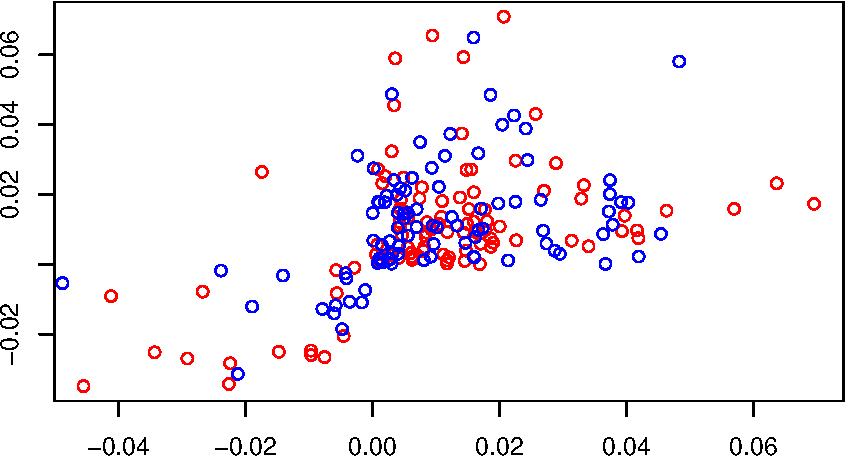
\includegraphics{hw4_files/figure-latex/unnamed-chunk-7-1.pdf}

\hypertarget{section-3}{%
\section{7.5}\label{section-3}}

Estimate the time-varying volatility matrix of the eight risk factors
presented in Example 7.5 using the last 3-month data and the estimator
(7.15) with \(\lambda =0.1\) (No estimate is needed for the initial 3
months). Present the results for the exchange rates and the S\&P 500
index, similar to Figure 7.3. Repeat the exercise by using the second
projection method in Section 7.2.2 and compare the results.

\begin{quote}
The eight risk factors include: (1) market risk, or the returns of the
S\&P 500; (2) volatility risk, or the VIX index; (3) exchange rate risk,
or the index of the US dollar value; (4) maturity risk, or the yield
spread between the 10 year US treasury and the 3 year treasury bills;
(5) default risk, or the yield spread between AAA and BBB corporate
bonds; (6) liquidity risk, or the difference between 1 month repo rates
and 1 month treasury bill rates; (7) size effect, or the difference of
returns between S\&P500 and Russell 2000; and (8) short term rate,
yields of the 3-month treasury bills.
\end{quote}

\begin{Shaded}
\begin{Highlighting}[]
\KeywordTok{library}\NormalTok{(quantmod)}
\NormalTok{start <-}\StringTok{ }\KeywordTok{as.Date}\NormalTok{(}\StringTok{"2018-08-01"}\NormalTok{)}
\NormalTok{end <-}\StringTok{ }\KeywordTok{as.Date}\NormalTok{(}\StringTok{"2018-11-01"}\NormalTok{) }\CommentTok{# getting the last 3 months data }
\CommentTok{# get the SPY  }
\KeywordTok{getSymbols}\NormalTok{(}\StringTok{"SPY"}\NormalTok{, }\DataTypeTok{from =}\NormalTok{ start, }\DataTypeTok{to =}\NormalTok{ end) }
\CommentTok{# get the US dollar value, exchange rate }
\KeywordTok{getSymbols}\NormalTok{(}\StringTok{"EUR=X"}\NormalTok{, }\DataTypeTok{src=}\StringTok{"yahoo"}\NormalTok{,}\DataTypeTok{from =}\NormalTok{ start, }\DataTypeTok{to =}\NormalTok{ end)}
\CommentTok{# get VIX}
\KeywordTok{getSymbols}\NormalTok{(}\StringTok{"^VIX"}\NormalTok{, }\DataTypeTok{src=}\StringTok{"yahoo"}\NormalTok{,}\DataTypeTok{from =}\NormalTok{ start, }\DataTypeTok{to =}\NormalTok{ end)}
\CommentTok{# get yield spread of 3 year and 10 year treasury bills }
\KeywordTok{getSymbols}\NormalTok{(}\StringTok{"T10Y3M"}\NormalTok{, }\DataTypeTok{src =} \StringTok{"FRED"}\NormalTok{, }\DataTypeTok{from =}\NormalTok{ start, }\DataTypeTok{to =}\NormalTok{ end) }
\CommentTok{# get default risk based on ICE BofAML US Corporate AAA and BBB Effective Yield}
\KeywordTok{getSymbols}\NormalTok{(}\StringTok{"BAMLC0A1CAAAEY"}\NormalTok{, }\DataTypeTok{src =} \StringTok{"FRED"}\NormalTok{, }\DataTypeTok{from =}\NormalTok{ start, }\DataTypeTok{to =}\NormalTok{ end)}
\KeywordTok{getSymbols}\NormalTok{(}\StringTok{"BAMLC0A4CBBBEY"}\NormalTok{, }\DataTypeTok{src =} \StringTok{"FRED"}\NormalTok{, }\DataTypeTok{from =}\NormalTok{ start, }\DataTypeTok{to =}\NormalTok{ end)}
\NormalTok{def <-}\StringTok{ }\NormalTok{BAMLC0A4CBBBEY }\OperatorTok{-}\StringTok{ }\NormalTok{BAMLC0A1CAAAEY}
\CommentTok{# get the liquidity risk, rely on fed funds rates as surrogate for repo  }
\KeywordTok{getSymbols}\NormalTok{(}\StringTok{"DGS1MO"}\NormalTok{, }\DataTypeTok{src =} \StringTok{"FRED"}\NormalTok{, }\DataTypeTok{from =}\NormalTok{ start, }\DataTypeTok{to =}\NormalTok{ end)}
\KeywordTok{getSymbols}\NormalTok{(}\StringTok{"DFF"}\NormalTok{, }\DataTypeTok{src =} \StringTok{"FRED"}\NormalTok{, }\DataTypeTok{from =}\NormalTok{ start, }\DataTypeTok{to =}\NormalTok{ end)}
\NormalTok{temp <-}\StringTok{ }\KeywordTok{merge.xts}\NormalTok{(DGS1MO, DFF)[}\StringTok{"2018-08-01/2018-11-01"}\NormalTok{]}
\NormalTok{liquidity <-}\StringTok{ }\NormalTok{temp}\OperatorTok{$}\NormalTok{DFF }\OperatorTok{-}\StringTok{ }\NormalTok{temp}\OperatorTok{$}\NormalTok{DGS1MO}
\CommentTok{# get the size effect }
\KeywordTok{getSymbols}\NormalTok{(}\StringTok{"^RUA"}\NormalTok{, }\DataTypeTok{src =} \StringTok{"yahoo"}\NormalTok{, }\DataTypeTok{from =}\NormalTok{ start, }\DataTypeTok{to =}\NormalTok{ end)}
\NormalTok{rua_returns <-}\StringTok{ }\KeywordTok{dailyReturn}\NormalTok{(RUA)}
\NormalTok{spy_returns <-}\StringTok{ }\KeywordTok{dailyReturn}\NormalTok{(SPY)}
\NormalTok{temp <-}\StringTok{ }\KeywordTok{merge.xts}\NormalTok{(rua_returns, spy_returns)}
\NormalTok{size <-}\StringTok{ }\NormalTok{temp}\OperatorTok{$}\NormalTok{daily.returns }\OperatorTok{-}\StringTok{ }\NormalTok{temp}\OperatorTok{$}\NormalTok{daily.returns}\FloatTok{.1}
\CommentTok{# get short term rate }
\KeywordTok{getSymbols}\NormalTok{(}\StringTok{"DGS3MO"}\NormalTok{, }\DataTypeTok{src =} \StringTok{"FRED"}\NormalTok{, }\DataTypeTok{from =}\NormalTok{ start, }\DataTypeTok{to =}\NormalTok{ end)}
\CommentTok{# combine all the returns }
\NormalTok{total <-}\StringTok{ }\KeywordTok{merge.xts}\NormalTok{(spy_returns, }\CommentTok{# market risk }
          \StringTok{`}\DataTypeTok{EUR=X}\StringTok{`}\NormalTok{[,}\DecValTok{4}\NormalTok{], }\CommentTok{# exchange risk }
\NormalTok{          VIX[,}\DecValTok{4}\NormalTok{], }\CommentTok{# volatility risk}
\NormalTok{          T10Y3M, }\CommentTok{# maturity risk }
\NormalTok{          def, }\CommentTok{# default risk }
\NormalTok{          liquidity, }\CommentTok{# liquidity risk}
\NormalTok{          size, }\CommentTok{# size effect }
\NormalTok{          DGS3MO) }\CommentTok{# short term rate }
\KeywordTok{names}\NormalTok{(total) <-}\StringTok{ }\KeywordTok{c}\NormalTok{(}\StringTok{"market"}\NormalTok{, }
                  \StringTok{"exchange"}\NormalTok{, }
                  \StringTok{"volatility"}\NormalTok{,  }
                  \StringTok{"maturity"}\NormalTok{, }
                  \StringTok{"default"}\NormalTok{, }
                  \StringTok{"liquidity"}\NormalTok{, }
                  \StringTok{"size"}\NormalTok{, }
                  \StringTok{"short"}\NormalTok{)}
\NormalTok{total <-}\StringTok{ }\KeywordTok{na.omit}\NormalTok{(total)}
\CommentTok{# make sure units make sense }
\NormalTok{total[,}\DecValTok{1}\NormalTok{] <-}\StringTok{ }\NormalTok{total[,}\DecValTok{1}\NormalTok{]}\OperatorTok{*}\DecValTok{100} \CommentTok{# convert to percent}
\NormalTok{total[,}\DecValTok{2}\NormalTok{] <-}\StringTok{ }\NormalTok{total[,}\DecValTok{2}\NormalTok{]}\OperatorTok{*}\DecValTok{100} \CommentTok{# convert exchange to percent }
\NormalTok{total[,}\DecValTok{7}\NormalTok{] <-}\StringTok{ }\NormalTok{total[,}\DecValTok{7}\NormalTok{]}\OperatorTok{*}\DecValTok{100} \CommentTok{# convert to basis pts  }
\CommentTok{# save }
\KeywordTok{saveRDS}\NormalTok{(total, }\StringTok{"~/workspace/st790-financial-stats/hw4/risk.rds"}\NormalTok{)}
\end{Highlighting}
\end{Shaded}

\begin{quote}
Now that we have aggregated all the necessary information, we can
calculate the time varying volatility matrix. First, the correlation
matrix:
\end{quote}

\begin{verbatim}
##            market exchange volatility maturity default liquidity   size
## market      1.000   -0.044     -0.346   -0.104   0.287    -0.136  0.228
## exchange   -0.044    1.000      0.535   -0.132   0.135     0.537  0.109
## volatility -0.346    0.535      1.000   -0.086  -0.275     0.410  0.061
## maturity   -0.104   -0.132     -0.086    1.000  -0.607     0.129 -0.041
## default     0.287    0.135     -0.275   -0.607   1.000    -0.149  0.138
## liquidity  -0.136    0.537      0.410    0.129  -0.149     1.000  0.267
## size        0.228    0.109      0.061   -0.041   0.138     0.267  1.000
## short      -0.174    0.304      0.805    0.045  -0.566     0.276 -0.025
##             short
## market     -0.174
## exchange    0.304
## volatility  0.805
## maturity    0.045
## default    -0.566
## liquidity   0.276
## size       -0.025
## short       1.000
\end{verbatim}

\begin{quote}
We can now apply thresholding to the correlation matrix:
\end{quote}

\begin{Shaded}
\begin{Highlighting}[]
\NormalTok{temp <-}\StringTok{ }\KeywordTok{cor}\NormalTok{(total)}
\NormalTok{temp2 <-}\StringTok{ }\NormalTok{temp}\OperatorTok{*}\KeywordTok{I}\NormalTok{(}\KeywordTok{abs}\NormalTok{(temp) }\OperatorTok{>}\StringTok{ }\FloatTok{.1}\NormalTok{)}
\KeywordTok{round}\NormalTok{(temp2, }\DecValTok{2}\NormalTok{)}
\end{Highlighting}
\end{Shaded}

\begin{verbatim}
##            market exchange volatility maturity default liquidity size
## market       1.00     0.00      -0.35    -0.10    0.29     -0.14 0.23
## exchange     0.00     1.00       0.53    -0.13    0.13      0.54 0.11
## volatility  -0.35     0.53       1.00     0.00   -0.27      0.41 0.00
## maturity    -0.10    -0.13       0.00     1.00   -0.61      0.13 0.00
## default      0.29     0.13      -0.27    -0.61    1.00     -0.15 0.14
## liquidity   -0.14     0.54       0.41     0.13   -0.15      1.00 0.27
## size         0.23     0.11       0.00     0.00    0.14      0.27 1.00
## short       -0.17     0.30       0.81     0.00   -0.57      0.28 0.00
##            short
## market     -0.17
## exchange    0.30
## volatility  0.81
## maturity    0.00
## default    -0.57
## liquidity   0.28
## size        0.00
## short       1.00
\end{verbatim}

\begin{Shaded}
\begin{Highlighting}[]
\NormalTok{n <-}\StringTok{ }\KeywordTok{nrow}\NormalTok{(total) }
\NormalTok{lambda <-}\StringTok{ }\FloatTok{.94} \CommentTok{# for daily }
\NormalTok{Sigma <-}\StringTok{ }\KeywordTok{array}\NormalTok{(}\DecValTok{0}\NormalTok{, }\KeywordTok{c}\NormalTok{(}\DecValTok{2}\NormalTok{, }\DecValTok{2}\NormalTok{, n}\OperatorTok{+}\DecValTok{1}\NormalTok{))}
\NormalTok{change <-}\StringTok{ }\KeywordTok{as.vector}\NormalTok{(}\KeywordTok{diff}\NormalTok{(total[, }\DecValTok{2}\NormalTok{])) }\CommentTok{# get the change for exchange rates }
\NormalTok{change[}\DecValTok{1}\NormalTok{] <-}\StringTok{ }\DecValTok{0}
\ControlFlowTok{for}\NormalTok{(i }\ControlFlowTok{in} \DecValTok{1}\OperatorTok{:}\NormalTok{n)\{}
\NormalTok{  tmp <-}\StringTok{ }\KeywordTok{as.numeric}\NormalTok{(}\KeywordTok{c}\NormalTok{(}\KeywordTok{as.numeric}\NormalTok{(total[i, }\DecValTok{1}\NormalTok{]), change[i]))}
\NormalTok{  Sigma[,,i}\OperatorTok{+}\DecValTok{1}\NormalTok{] <-}\StringTok{ }\NormalTok{lambda}\OperatorTok{*}\NormalTok{Sigma[,,i] }\OperatorTok{+}\StringTok{ }\NormalTok{(}\DecValTok{1}\OperatorTok{-}\NormalTok{lambda)}\OperatorTok{*}\NormalTok{tmp }\OperatorTok\StringTok{ }\KeywordTok{t}\NormalTok{(tmp)}
\NormalTok{\}}
\NormalTok{Sigma <-}\StringTok{ }\NormalTok{Sigma[,,}\OperatorTok{-}\DecValTok{1}\NormalTok{] }\CommentTok{# remove the initial values }
\NormalTok{leverage <-}\StringTok{ }\NormalTok{Sigma[}\DecValTok{1}\NormalTok{,}\DecValTok{2}\NormalTok{,]}\OperatorTok{/}\KeywordTok{sqrt}\NormalTok{(Sigma[}\DecValTok{1}\NormalTok{,}\DecValTok{1}\NormalTok{,])}\OperatorTok{/}\KeywordTok{sqrt}\NormalTok{(Sigma[}\DecValTok{2}\NormalTok{,}\DecValTok{2}\NormalTok{,]) }
\CommentTok{# present the results like 7.3 }
\KeywordTok{par}\NormalTok{(}\DataTypeTok{mfrow =} \KeywordTok{c}\NormalTok{(}\DecValTok{2}\NormalTok{,}\DecValTok{2}\NormalTok{), }\DataTypeTok{mar=}\KeywordTok{c}\NormalTok{(}\DecValTok{4}\NormalTok{,}\DecValTok{2}\NormalTok{,}\DecValTok{2}\NormalTok{,}\DecValTok{1}\NormalTok{)}\OperatorTok{+}\FloatTok{0.1}\NormalTok{, }\DataTypeTok{cex=}\FloatTok{0.8}\NormalTok{)}

\KeywordTok{plot}\NormalTok{(}\KeywordTok{sqrt}\NormalTok{(Sigma[}\DecValTok{1}\NormalTok{,}\DecValTok{1}\NormalTok{,]), }\DataTypeTok{type=}\StringTok{"l"}\NormalTok{, }\DataTypeTok{col=}\DecValTok{4}\NormalTok{, }\DataTypeTok{xlab =} \StringTok{""}\NormalTok{)}
\KeywordTok{title}\NormalTok{(}\StringTok{"Daily volatility of SP500 Returns"}\NormalTok{)}

\KeywordTok{plot}\NormalTok{(}\KeywordTok{sqrt}\NormalTok{(Sigma[}\DecValTok{2}\NormalTok{,}\DecValTok{2}\NormalTok{,]), }\DataTypeTok{type=}\StringTok{"l"}\NormalTok{, }\DataTypeTok{col=}\DecValTok{4}\NormalTok{, }\DataTypeTok{xlab =} \StringTok{""}\NormalTok{)}
\KeywordTok{title}\NormalTok{(}\StringTok{"SD of changes of exchange rates"}\NormalTok{)}

\KeywordTok{plot}\NormalTok{(leverage, }\DataTypeTok{type=}\StringTok{"l"}\NormalTok{, }\DataTypeTok{col=}\DecValTok{4}\NormalTok{, }\DataTypeTok{ylim=}\KeywordTok{c}\NormalTok{(}\OperatorTok{-}\DecValTok{1}\NormalTok{,}\DecValTok{0}\NormalTok{), }\DataTypeTok{xlab =} \StringTok{""}\NormalTok{)}
\KeywordTok{title}\NormalTok{(}\StringTok{"Correlation of SPX returns and exchange rates"}\NormalTok{)}

\KeywordTok{plot}\NormalTok{(leverage, Sigma[}\DecValTok{2}\NormalTok{,}\DecValTok{1}\NormalTok{,], }\DataTypeTok{type=}\StringTok{"l"}\NormalTok{, }\DataTypeTok{col=}\DecValTok{4}\NormalTok{, }\DataTypeTok{xlab =} \StringTok{""}\NormalTok{)}
\KeywordTok{title}\NormalTok{(}\StringTok{"Covariance of SPX returns and exchange rates"}\NormalTok{)}
\end{Highlighting}
\end{Shaded}

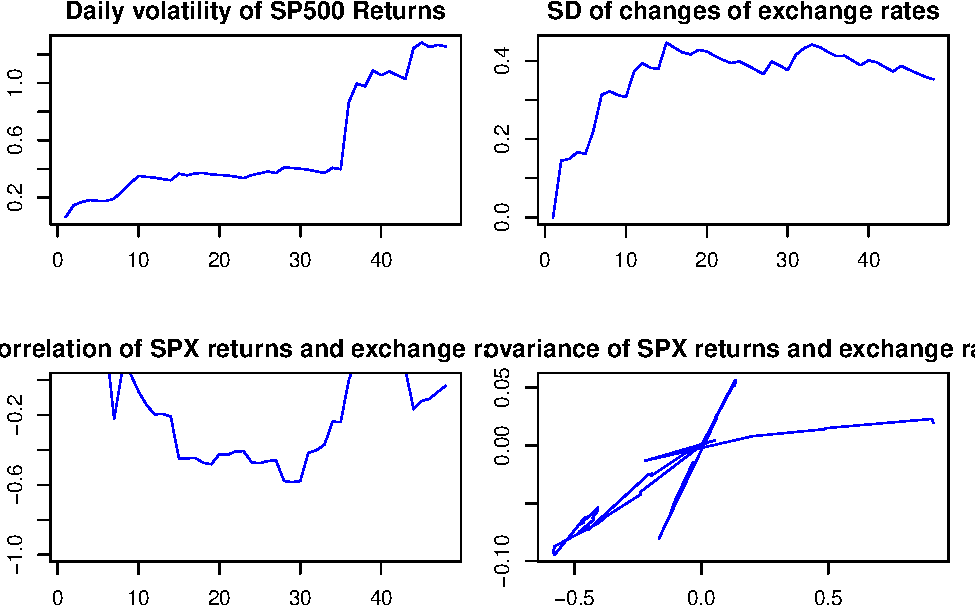
\includegraphics{hw4_files/figure-latex/unnamed-chunk-11-1.pdf}

\begin{quote}
Using the second projection method, we want to compute: \[
\hat{\Sigma}_{\lambda}^\texttt{+} = (\hat{\Sigma}_{\lambda} + \lambda_{\min{}}^\texttt{-} I_p) / (1+\lambda_{\min}^\texttt{-})
\]
\end{quote}

\begin{Shaded}
\begin{Highlighting}[]
\CommentTok{# find the eigenvalues }
\NormalTok{min_eigen <-}\StringTok{ }\KeywordTok{numeric}\NormalTok{(n)}
\ControlFlowTok{for}\NormalTok{(i }\ControlFlowTok{in} \DecValTok{1}\OperatorTok{:}\NormalTok{n)\{}
\NormalTok{  eigenval <-}\StringTok{ }\KeywordTok{eigen}\NormalTok{(Sigma[,,i])}\OperatorTok{$}\NormalTok{values}
\NormalTok{  min_eigen[i] <-}\StringTok{ }\KeywordTok{min}\NormalTok{(eigenval)}
\NormalTok{\}}
\end{Highlighting}
\end{Shaded}

\begin{quote}
Since the \(\lambda_{\min}^\texttt{-}\) factor is always 0, our
estimates do not change, and we have the same results as if we simply
utilized the thresholding technique.
\end{quote}
\newpage
\singlespacing 
\end{document}
